% Chapter 5

\chapter{Identification and Authentication} 
\label{Chapter5}
\lhead{Chapter 5. \emph{Identification and Authentication}}

\section{Overview and Intentions}

In this chapter we will be discussing the methods used by one entity to verify that the identity given by another is valid. This is often referred to as identification, or entity authentication. We say that the \emph{verifier} is requesting assurance that the \emph{claimant's} identity is actually what the claimant has defined. We also must define \emph{timeliness} as part of entity authentication: the claimant's identity can only be verified during the execution of the identification protocol in real-time, this is known as a \emph{lively correspondence}.

The main type of authentication that we will be looking at, particularly for the Enigma application, is \emph{authenticated key establishment}. Often entity authentication protocols are used not only to verify identity, but also to further secure transmissions. For example, as we have discussed extensively, keys need to be shared securely and thus we also need methods for proving that a received key is from the entity with which we want to communicate. 

\section{Digital Signatures}

  \subsection{Overview}
  
  A digital signature is often compared to real life signatures, a verification of identity, however this is not entirely true. A digital signature is comparable to a handwritten signature in the way that someone could handwrite a signature on a document to prove that it is valid and (perhaps in this example) written by them. The use of digital signatures extends further than this, and can be defined in terms of information security as listed in \textsection\ref{Chapter2}:
  
  \begin{enumerate}
    \item Authentication -- the document comes from the expected entity (assuming the public keys can be trusted).
    \item Integrity -- a digital signature acts as a way of checking that the received data matches the data that was signed and transmitted.
    \item Non-repudiation -- a signed document cannot be revoked and the sending entity cannot claim they did not sign it.
  \end{enumerate}
  
  This of course introduces a chicken-and-egg issue: how do you verify the identity of someone without having them digitally sign proof of their identity? This is solved by the use of trusted third parties and certificates (\textsection\ref{sec:certs}) -- that is to say, having \emph{another entity} sign proof of the sender's identity.
  
  There are two overall types of digital signature algorithms: those with \emph{appendices}, and those with \emph{message recovery}. Generally signatures with appendix are more common.
  
  \begin{enumerate}
    \item With Appendix -- reliant on cryptographic hash functions to provide message summaries that can be signed and then compared to summaries of the received document.
    \item With Message Recovery -- the message signed can be recovered from the signature, which is typically of use only for short messages.
  \end{enumerate}
  
  We will be using a scheme with appendix: RSA.
  
  An example of a transmission between two entities, Alice and Bob, is given to show the process of signing and verifying messages.
  
  \begin{enumerate}
    \item Alice creates a message $M$ and signs it using her private key known only to her, producing signature $S$, sending both to Bob.
    \item Bob receives $\{S,M\}$ and retrieves Alice's public key.
    \item Bob verifies that $M$ is unmodified (integrity) and from Alice (authentication) by comparing it to $S$ using a pre-defined method.
  \end{enumerate}
  
  Signatures are a simple but secure method of ensuring information security.
  
  \subsection{RSA}
  
  The RSA digital signature scheme was the first feasible scheme to be introduced, and remains the most popular. It works in very much the same way as RSA public-key encryption/decryption: through the generation of an exponent and modulus to be used in a bijective formula where the exponents are reversed for encryption/decryption.
  
  \paragraph{Why use RSA?} It is the most prevalent algorithm for message signing, and as we have covered the theory already it should be easy to understand and link in with our existing key infrastructure.
  
  \subsubsection{Algorithm}
  
  Key generation is the same as in \textsection\ref{subsubsec:rsa_keygen}.
  
  \begin{enumerate}
    \item Signing (Alice):
    \begin{enumerate}
      \item Convert message $m$ in to an integer representative.
      \item Calculate $s = m^d \mod N$, where $d$ is the private exponent, and $N$ the modulus.
      \item Attach $s$ to the message $m$ and transmit $\{s,m\}$.
    \end{enumerate}
    \item Verification (Bob):
    \begin{enumerate}
      \item Receive $\{s,m\}$ and obtain Alice's public key.
      \item Calculate $em = s^e \mod N$, where $e$ is Alice's public exponent.
      \item If $em$ matches $m$, then $m$ is valid.
    \end{enumerate}
  \end{enumerate}
  
  \subsubsection{Implementation}
  
    This is trivial to implement, however as with RSA encryption/decryption the standard algorithm is susceptible to several attacks. Our previous scheme -- OAEP -- is not applicable for use in digital signatures and so we will be using a scheme known as RSA-PSS: RSA Probabilistic Signature Scheme. Approved in 2003 as an RFC\cite{Jonsson:2003aa}, it is now the accepted standard to be used for digital signatures utilising the RSA algorithm.
    
    The scheme adds two well-defined methods in to the algorithm: \verb!EMSA-PSS-ENCODE!, an algorithm to format data before mathematically signing it, and \verb!EMSA-PSS-VERIFY! an algorithm that verifies the signature \emph{after} it has been mathematically verified using RSA. To better describe the scheme, we also define two methods as displayed in the RFC\cite{Jonsson:2003aa}: \verb!RSASP1! produces a signature representative of a message $m$, and \verb!RSAVP1! returns a message representation of a given signature $s$.
    
    Signing a message $m$ now works as so:
    
    \begin{enumerate}
      \item Encode the message: \verb!EMSA-PSS-ENCODE(m)!.
      \item Convert the message to an representative integer form: \verb!OS2IP(m)!.
      \item Using a private key $p$, calculate the signature representative $s$ using RSA: \verb!RSASP1(p,m)!.
      \item Convert the signature (integer) representative back to a byte string: \verb!I2OSP(s)!.
    \end{enumerate}
    
    Verification is the reverse, with the method change as described above. Given a signature $s$:
    
    \begin{enumerate}
      \item Convert $s$ into an integer representative: \verb!OS2IP(s)!.
      \item Using public key $p$, calculate the message representative $m$: \verb!RSAVP1(p,s)!
      \item Convert $m$ to a byte string: \verb!I2OSP(m)!.
      \item Verify the byte string using \verb!EMSA-PSS-VERIFY!.
    \end{enumerate}
    
    Indeed, \cite{Alfred-Menezes:1996kx} shares a simplified diagram of how the processes work:
    
    \begin{center}
      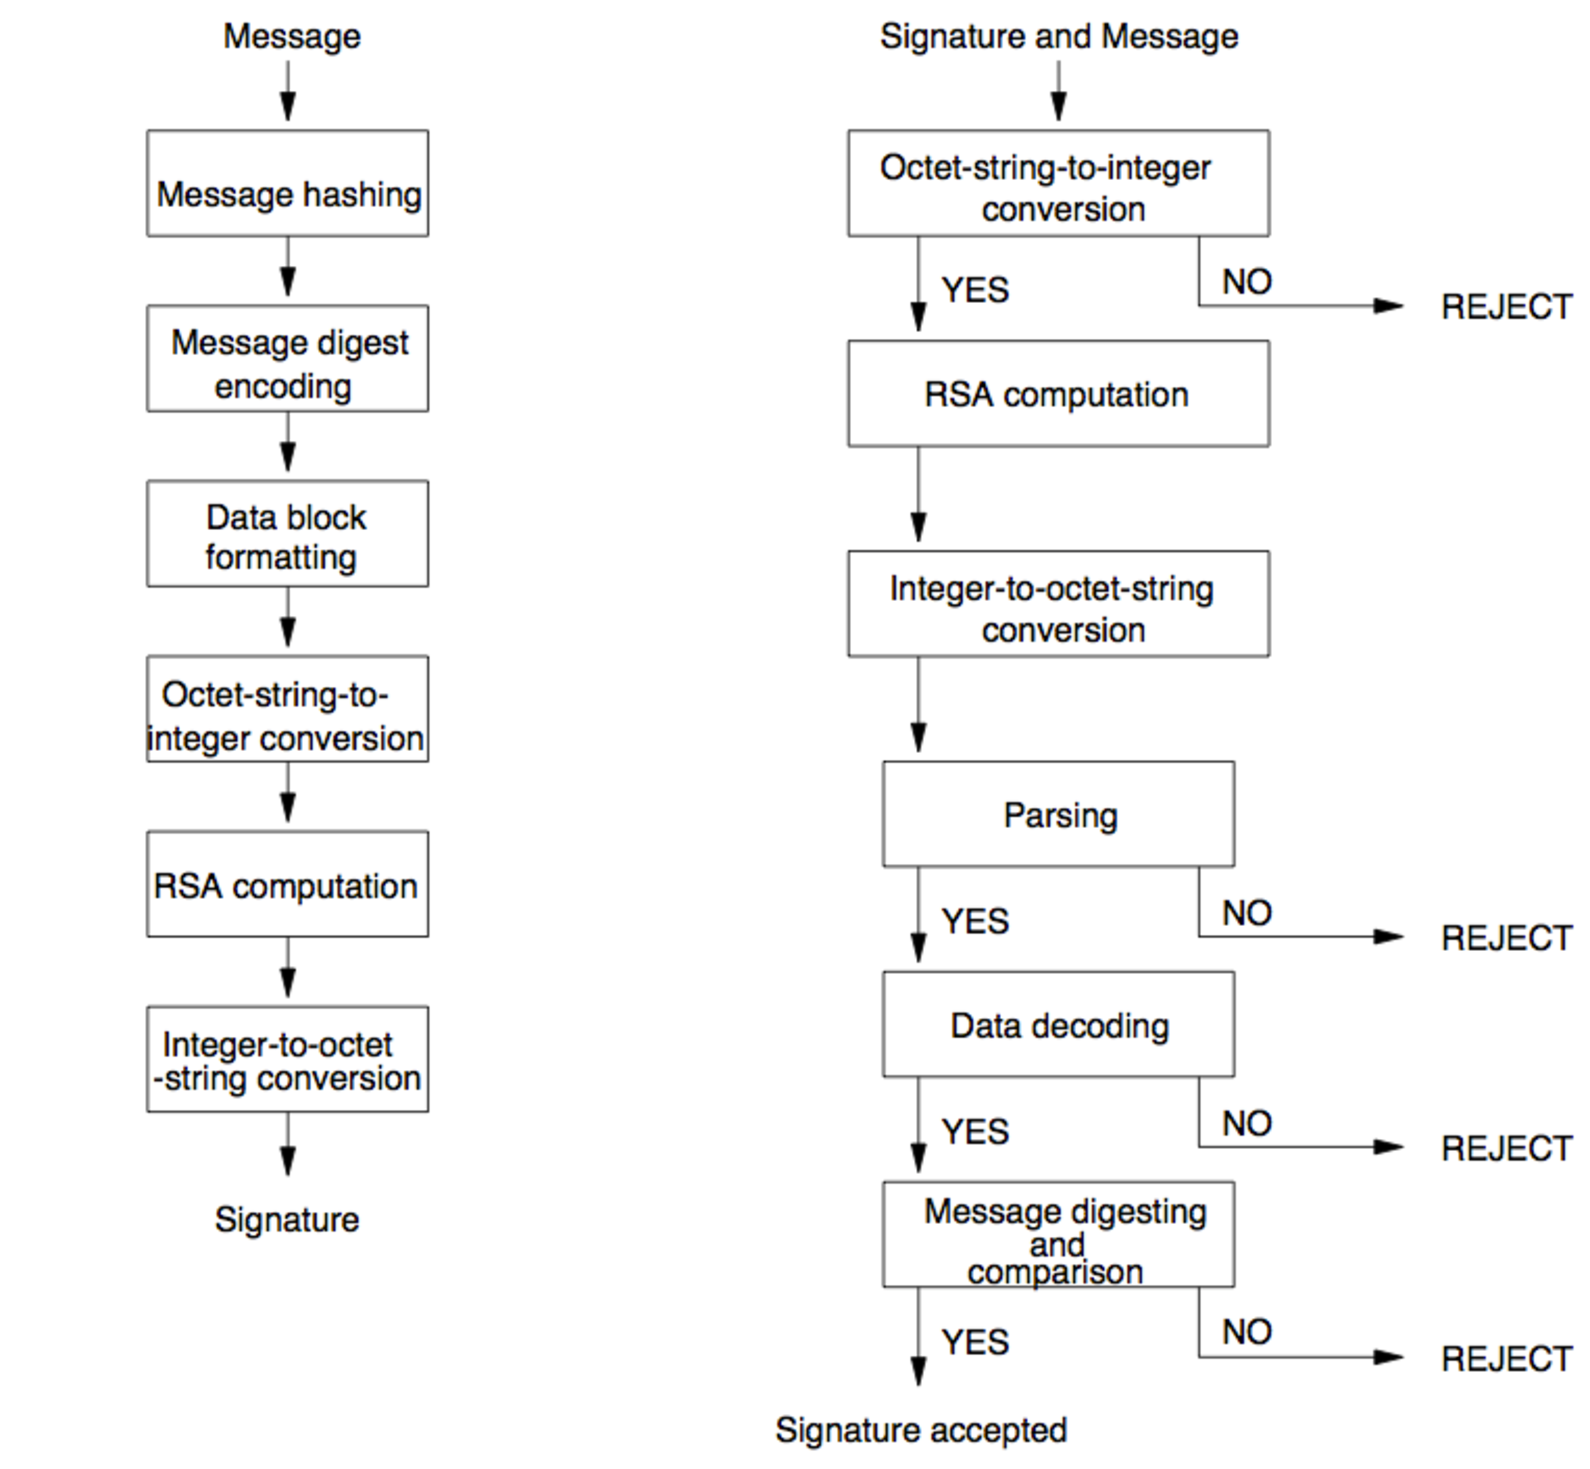
\includegraphics[scale=0.5]{./Figures/Ch5/5-2-2-2.pdf}
    \end{center}
    
    \cite{Jonsson:2003aa} makes one (unstated) point: good reference documentation for an algorithm will almost always result in a robust implementation. This RFC gives an excellent overview and exact requirements for the algorithm, meaning that our implementation process is relatively pain-free.
    
    \paragraph{RSA Primitives} are of course the simplest. Recall that given an exponent $e$ -- be it private or public -- and modulus $N$, we have $m = c^e \mod N$. Interestingly, this means we only have to implement the actual code once and the other primitive can simply override this method for naming convention as both public and private exponents are large integers and can be swapped interchangeably. \\
    
    \begin{lstlisting}
private BigInteger RSASP1(BigInteger m) {
  // 2. Let s = m^d mod n.
  BigInteger s = m.modPow(E, N);
  return s;
}

private BigInteger RSAVP1(BigInteger s) {
  // 2. Let m = s^e mod n.
  return this.RSASP1(s);
}
\end{lstlisting}
 
    Once again we are using the \verb!BigInteger! class for storing large integers (see \textsection\ref{subsubsec:fermat}).
    
    Before discussing the implementation of the EMSA--PSS functionality, we must first define how they actually work.
    
    \paragraph{EMSA--PSS--ENCODE} differs from the original signature-with-appendix scheme created by Bellare and Rogaway, almost entirely in the small details. For example, applying a hash function instead of a mask generation function. 
    
    The structure of the final encoded string is somewhat similar to that in RSA--OAEP \cite{Jonsson:2003aa}. \\
    
    \begin{center}
\lstset{stringstyle={},numbers=none}
\begin{lstlisting}
                                  +-----------+
                                  |     M     |
                                  +-----------+
                                        |
                                        V
                                      Hash
                                        |
                                        V
                          +--------+----------+----------+
                     M' = |Padding1|  mHash   |   salt   |
                          +--------+----------+----------+
                                         |
               +--------+----------+     V
         DB =  |Padding2|   salt   |   Hash
               +--------+----------+     |
                         |               |
                         V               |    +--+
                        xor <--- MGF <---|    |bc|
                         |               |    +--+
                         |               |      |
                         V               V      V
               +-------------------+----------+--+
         EM =  |    maskedDB       |     H    |bc|
               +-------------------+----------+--+
\end{lstlisting}
    \end{center}

    \begin{enumerate}
      \item A message $M$ is hashed, and then this hash is concatenated with eight zero-bytes (\verb!Padding1!) and a random-byte string, with length equal to the digest length of the hash function, known as a salt.
      \item A byte array $DB$ is created, consisting of a padding string and the salt, separated by the byte \verb!0x01!.
      \item A mask generation function (\textsection\ref{subsubsec:oaep}) is used to mask the hashed message to a length of (the maximum size \verb!BigInteger! - the maximum hash length - 1), which is then XOR'd with $DB$.
      \item The final string is the masked $DB$ with the hashed message and a byte \verb!0xbc!.
    \end{enumerate}

    Due to the length of the code, it is recommended that it is viewed electronically, and can be found at \emph{com.cyanoryx.uni.crypto.rsa.RSA\_PSS}.
    
    \paragraph{Given the message} $M$ and encoded message $EM$, EMSA--PSS-VERIFY works similarly in that it encodes the given message and compares the computed signatures to the one received, along with some interstitial error checking to remove unnecessary calculation if the verification fails early on (for example, in correct padding separator bytes).
    
    \begin{enumerate}
      \item Hash the message so $H = M$, and check to see if the rightmost byte of $EM$ is \verb!0xbc!.
      \item Create $maskedDB$ to be (the maximum size \verb!BigInteger! - the maximum hash length - 1) bits of $EM$ and the next (maximum hash length) bits of $M$.
      \item Mask the hash of $M$ to be (the maximum size \verb!BigInteger! - the maximum hash length - 1) bits, and XOR it with $maskedDB$, creating $DB$.
      \item Let \verb!salt! be the last $n$ bytes of of $DB$ where $n$ is a predefined salt length.
      \item Create the byte array $M'$ such that \\ $M = $ \verb!(0x) 00 00 00 00 00 00 00 00 || Hash(!$M$\verb!) || salt!.
      \item Let $H' = Hash(M')$ and if $H = H'$, the signature is valid, otherwise not.
    \end{enumerate}
    
    \paragraph{Keys} are handled using the same infrastructure as RSA--OAEP. A \verb!Key! object with descendants \verb!PrivateKey! and \verb!PublicKey! store the exponent and modulus, and is passed in when the \verb!RSA_PSS! object is first instantiated. This means that keys stored on disk or in memory can be imported without the developer parsing them manually.

\section{Certificates}
\label{sec:certs}

  \subsection{Overview}
  
  Now that we understand digital signatures, we can address an issue with their use: how can you verify that the public key you are using is the key belonging to the entity you believe you are receiving communications from. The scenario is as so: 
  
  \begin{enumerate}
    \item Alice creates and signs a message $m$, sending Bob the signature $s$ with it: $\{s,m\}$.
    \item Mallory intercepts the message, modifies it, and signs it using her own private key and sends it to Bob.
    \item Bob received the message, and obtains Alice's public key. However, Mallory -- the means through which she does it are not relevant -- has replaced Alice's public key with her own.
    \item Bob now verifies Mallory's message, believing that it has come from Alice and has not been changed.
  \end{enumerate}
  
  A commonly used concept in cryptography is the \emph{trusted third party} (TTP). In this case, an entity with whom we place trust to act as an arbiter or facilitator between us and other entities to mutually verify identity. In the case of certificates, a TTP is known as a Certificate Authority (CA) and our trust in them is based on a \emph{chain} that is bundled with operating systems and web browsers. This chain consists of the public keys of the CAs, which can be used to verify the keys of other entities, however we will discuss this further below. These trusted third parties are the most widely used solution to the problem of ensuring that received public-keys match with the entity we expect.
  
  Keypair owners pay Certificate Authorities to accept their public keys and proofs of identity (some form of ID, bank statements, proof of address, etc.) so that they can sign the keypair owner's public key and distribute the signature so that other entities may verify this signature and key, thus proving it belongs to the designated person.
  
  However, we need a way of distributing all this information in a standardised way -- certificates. The current standard used for structuring the data stored in certificates is known as \emph{X.509v3}\cite{Cooper:2008aa}. This defines a rigid structure that X.509 certificates must follow, such as in what order to include the subject's (entity's) name, key, signature, etc. and how to do so.
  
  \subsection{Enigma Certificates}
  
  As part of our testbed we will be implementing a version of the X.509v1 specification\cite{Kent:1993aa}: \\
  
  \begin{lstlisting}
Cert { Algorithm, Signature },
CertDetails {
  Issuer,
  Serial,
  Validity { notBefore, notAfter },
  UniqIdent,
  SubjectInfo { Name, Algorithm, Public Key }
}
  \end{lstlisting}
  
  We create a class \verb!Certificate! for storing this information, as well as handling certificate files and exporting them. Within this class, Certificates are stored locally within private \verb!byte[]! fields, and are passed to the class using a \verb!java.util.HashTable<String,byte[]>! so that multiple parameter handling is not needed on either end.
  
  Outside of the class, certificates are stored in a pre-defined ASCII format (items enclosed in square brackets represent a field to be filled with data): \\
  
  \lstset{commentstyle={}}
  \begin{lstlisting}
-----BEGIN-ENIGMA-CERTIFICATE----- \n
[SignatureAlgorithm],[Signature]//[Issue]|[Serial]|
[ValidityNotBefore],[ValidityNotAfter]|[UniqIdent]|
[SubjectName],[SubjectAlgorithm],[SubjectKey] \n
-----END-ENIGMA-CERTIFICATE-----
\end{lstlisting}

  We provide two constructors: \verb!Certificate(String c)! that automatically parses the data provided in to a \verb!Certificate! object, and \verb!Certificate(File c)! that reads a file in then passes it to \verb!Certificate(String c)! for processing.
  
  Alongside this \verb!toString()! is overridden to output the certificate in a writeable form, and \verb!toReadable()! to output the certificate in a text form that is readable by a user.
  
  The details of this class can be found at \emph{com.cyanoryx.uni.crypto.cert.Certificate}, and are not listed here to the simplicity of its operation.
  
  \subsubsection{Certificate Authority}
  
  This is no use, however, without a trusted third party to sign the keys in the certificate. We create a utility class, \verb!CertificateAuthority!, that signs keys and verifies certificates using the \verb!Certificate! class and RSA-PSS. \\
  
  \begin{lstlisting}
public boolean verify(Certificate cert) throws DataFormatException {
  byte[] signature = cert.getSignature();
  byte[] key     = cert.getSubject_key();
  
  RSA_PSS rsa = new RSA_PSS(this.pub);
  return rsa.verify(key, signature);
}

public byte[] sign(byte[] key) throws DataFormatException {
  if (this.priv==null) throw new DataFormatException("No private key found");
  
  RSA_PSS rsa = new RSA_PSS(this.priv);
  return rsa.sign(key);
}
\end{lstlisting}

\section{Summary}

With certificates and digital signatures, the flow of encryption and decryption when sharing messages is different:

\begin{enumerate}
  \item Bob sends his public-key certificate to Alice.
  \item Alice verifies Bob's public key in his certificate by using the certificate authority's public key.
  \item Alice generates a session key $k$, and encrypts it using Bob's public key and transmits it to him.
  \item Bob decrypts the session key and now both entities have a share secret key.
\end{enumerate}